%\documentclass{book}
%\begin{document}
\chapter{Definizione del problema}
\setcounter{section}{1}
(replicazione dei dati - introduzione)
\item
\subsection{Cluster di database}
Un cluster \`{e} una raccolta di componenti che garantisce scalabit\`{a} e disponibilit\`{a} distribuendone i costi. Un cluster di database (SQL usa il termine cluster di catalogo) \`{e} una collezione di database gestiti da una singola istanza di un server database in esecuzione. Un'istanza \`{e} la raccolta di memoria e processi che interagiscono con un database, cio\`{e} l'insieme di file fisici che effettivamente memorizzano i dati.\cite{etichetta1} A tal fine, \`{e} possibile creare un cluster di database per applicazioni enterprise high-end, memorizzando e elaborando informazioni sui nodi.\\ L'architettura per un cluster di database \`{e} distinta da come le responsabilit\`{a} dei dati sono condivise tra i nodi di calcolo.

Seguono due dei vantaggi principarli offerti dal clustering, specialmente in un ambiente di database di alto volume:
\begin{itemize}
\item 
Fault tolerance (tolleranza di guasti): in caso di guasto del singolo server, il cluster offre un'alternativa, poich\'{e} esiste pi\`{u} di un server o istanza per gli utenti a cui connettersi.
\item
Load balancing (bilanciamento del carico): la funzionalit\`{a} di clustering \`{e} generalmente impostata per consentire agli utenti di essere assegnati automaticamente al server con il minor carico.\cite{etichetta1} 
\end{itemize}
Ci sono differenti tipi di architetture clustering, che si diversificano da come vengono memorizzati i dati e allocate le risorse.
La prima modalit\`{a} di clustering \`{e} conosciuta come architettura "Shared-Nothing" (SN). \`{E} un'architettura di elaborazione distribuita in cui ogni nodo/server \`{e} totalmente indipendente e autonomo, pertanto nessuno dei nodi condivide memoria o archiviazione del disco. Pi\`{u} generalmente, non esiste un unico punto di contesa nel sistema.\cite{etichetta5} Il partizionamento \`{e} tale che ogni nodo possiede un sottoinsieme dei dati, ovvero ogni nodo ha accesso esclusivo su quel particolare sottoinsieme. 
((Un esempio di questa forma di clustering potrebbe essere quando un'azienda ha pi\`{u} data centers per un unico sito web. Con molti server in tutto il mondo, nessun singolo server \`{e} un "master".\cite{etichetta2}))\\

\begin{figure}[htbp]
\centering
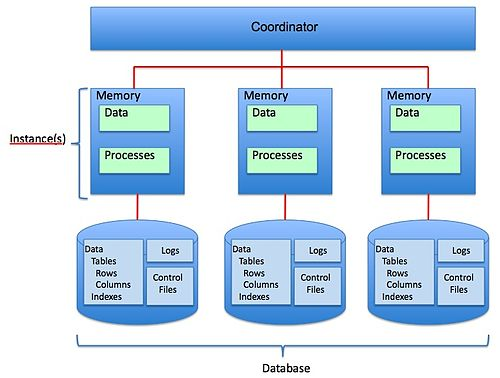
\includegraphics[scale=0.70]{img/Shared_Nothing_Architecture.jpg}\\
\caption{Architecture Shared Nothing \label{figura1.1} \cite{etichetta7}}
\end{figure}

I vantaggi dell'architettura SN rispetto a un'entit\`{a} centrale che controlla la rete (un'architettura basata su controller) riguarda l'eliminazione di qualsiasi singolo punto di guasto, consentendo funzionalit\`{a} di (self-healing) auto-riparazione e fornendo un vantaggio nell'offrire aggiornamenti non distruttivi.\cite{etichetta6} 
\textbf{DA LEGGERE PER BENE ARTICOLO CITATO.}
Shared-nothing \`{e} anche noto come "database sharding". In generale, un sistema SN divide i suoi dati in vari nodi su database diversi o pu\`{o} richiedere a ciascun nodo di mantenere la propria copia dei dati dell'applicazione utilizzando un qualche tipo di protocollo di coordinamento.\cite{etichetta5}\\
Si oppone a quest'ultima, l'architettura nota come "shared-disk" (disco condiviso), in cui tutti i dati vengono memorizzati centralmente in un unico disco e sono accessibili da tutti i nodi di cluster.\cite{etichetta7} In questo tipo di struttura quindi pi\`{u} istanze di database vengono raggruppate in un singolo database sul disco. Nei sistemi di dischi condivisi, i blocchi (o pagine) di dati su disco possono avere un solo proprietario.((
La proprietà dei blocchi (o pagine) viene trasferita all'istanza che sta facendo l'aggiornamento. Questo genera traffico di rete e in genere un'infrastruttura dedicata viene implementata tra le istanze di database per far fronte a questo traffico.))
L'architettura Shared-Disk \`{e} un esempio di Synchronous Multi-Master, ovvero ogni istanza del database pu\`{o} scrivere (cio\`{e} \`{e} un master) in modo sincrono.\cite{etichetta7}
\textbf{DA CHIEDERE E DA CONTROLLARE ULTIME FRASI. GUARDA COMMENTO per il sito}
%https://en.wikibooks.org/wiki/Oracle_and_DB2,_Comparison_and_Compatibility/Database_Scaling/Shared_Architectures}}

\begin{figure}[htbp]
\centering
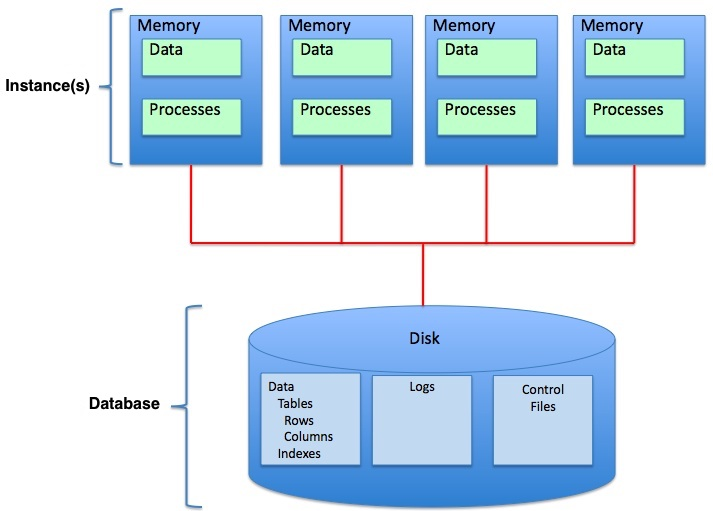
\includegraphics[scale=0.40]{img/Shared_Disk_Architecture.jpg}\\
\caption{Architecture Shared Disk - Shared Everything \label{figura1.2} \cite{etichetta7}}
\end{figure}

In un'architettura SD, grandi reti di computer possono operare su un singolo set di dati senza la necessit\`{a} di replicare o bloccare quel set di dati.\cite{etichetta7}
Shared Disk ha due vantaggi: ogni processore ha la propria memoria, il bus di memoria non \`{e} un collo di bottiglia (contrariamente all'architettura "Shared-Everything"). Inoltre il sistema offre un modo semplice per fornire un certo grado di tolleranza agli errori.\\

((La distinzione tra i due tipi \`{e} diventata confusa di recente con l'introduzione di grid computing o distribuzione cache. In questa configurazione, i dati sono ancora gestiti centralmente, ma controllati da un potente "server virtuale" composto da molti server che lavorano insieme come uno.\cite{etichetta2}))
\item
\subsection{Rete di pari}

\item
\subsection{Sistemi di ridondanza disco (RAID)}
RAID, acronimo di "redundant array of independent disks", insieme ridondante di dischi indipendenti, (originariamente "redundant array of inexpensive disks"), \`{e} un modo per memorizzare gli stessi dati in luoghi diversi su pi\`{u} dischi rigidi per proteggere i dati nel caso di un guasto di unit\`{a}. Tuttavia, non tutti i livelli RAID forniscono la ridondanza.
\textbf{History of RAID?}
Il RAID funziona mettendo i dati su pi\`{u} dischi e consentendo operazioni di input/output (I/O) di sovrapporsi in modo equilibrato, migliorando le prestazioni. Poich\'{e} l'utilizzo di pi\`{u} dischi aumenta il tempo medio tra i guasti (MTBF), memorizzare dei dati ridondantemente aumenta anche la tolleranza agli errori.
\item
\subsection{Codice di correzione errore (erasure coding)}
\textbf{http://searchstorage.techtarget.com/definition/erasure-coding}
\item
\section{Hardware utilizzato per gli esperimenti}
\textbf{Inserire foto hardware con descrizione}
\item
\section{Software utilizzato per gli esperimenti}
\item
\subsection{PosgreSQL}

\textbf{(spiegazione cinci -audio-)}
Uno dei punti di forza che ha reso famoso e versatile Posgres è che è un DBMS (Database Management System è un sistema software progettato per consentire la creazione e manipolazione efficiente di database (ovvero di collezioni di dati strutturati) ) (scritto in C). Ha dei rametti dove te riesci ad agganciarci dei software fatti ad OC. te ti agganci a un sistema di segnalistica interna e lui quindi tramite messaggi di scambio interno ti permette di lavorare (ti dice "ho fatto l'inserimento di questa tabella(INSERT), ti scatta il segnale, e te riesci a intercettare e quindi fare delle operazioni)

Pg Logical è un estensione di Posgres. Lui capisce quando fa inserimenti e riesce a duplicare soltando parti di database. Mentre replica di posgres per adesso ti replicherebbe tutto il DB. Invece noi si fa con solo tabelle (R) o quanti record di tabelle (per id maggiori di x) adirittura si vogliono replicare o colonne di tabelle \\
\textbf{(spiegazione cinci -audio-)}


Con il termine PostgreSQL viene denominato un particolare ORDBMS, acronimo di Object-Relational DataBase Management System, cioè un software relazionale e ad oggetti per la gestione di basi di dati.
PostgreSQL è Open Source, quindi il suo codice sorgente è disponibile pubblicamente ed "aperto" ai contributi degli sviluppatori che volontariamente intendono partecipare alla sua implementazione.

In PostgreSQL, ma il discorso può essere allargato a tutti i gestori di database relazionali, i dati vengono rappresentati attraverso delle tabelle e le tabelle sono gestite utilizzando un linguaggio di alto livello chiamato SQL, acronimo di Structured Query Language.
Nel caso specifico, l'ORDBMS avrà il compito di gestire le operazioni di archiviazione e di salvaguardia dell'integrità dei dati allocati.

L'SQL è quindi un linguaggio a disposizione dell'utente da impiegare per "interfacciarsi" ai gestori di database; esso ha la caratteristica di agire in modo "trasparente", infatti le operazioni svolte a carico dei dati saranno portate avanti senza bisogno che l'utilizzatore sappia in che modo essi vengono trattati.\\
\textbf{(spiegazione cinci -audio-}\\
\textbf{(http://www.slony.info/images/Slony-I-concept.pdf}\\
Replicating schema changes is an often discussed problem and only ver y
fe w database systems provide the necessary hooks to implement it. PostgreSQL
does not provide the ability to define triggers called on schema changes, so a
transparent way to replicate schema changes is not possible without substantial
work in the core PostgreSQL system.
Moreover, ver y often database schema chages are not single, isolated DDL
statements that can occur at any time within a running system. Instead they tend
to be groups of DDL and DML statements that modify multiple database objects
and do mass data manipulation like updating a new column to its initial value.
The Slony-I replication system will have a mechanism to execute SQL
scr ipts in a controlled fashion as part of the replication process.

\item
\subsection{Concept Provider-Subscriber}
Master to multiple cascaded slaves
The basic structure of the systems combined in a Slony-I installation is a
master with one or more slaves nodes. Not all slave nodes must receive the replication
data directly from the master. Every node that receives the data from a
valid source can be configured to be able to forward that data to other nodes.
There are three distinct ideas behind this capability. The first is scalability.
One database, especially the master that receives all the update transactions
from the client applications, has only a limited capability to satisfy the slave
nodes queries during the replication process. In order to satisfy the need for a big
number of read-only slave systems it must be possible to cascade.
The second idea is to limit the required networ k bandwidth for a backup site
while keeping the ability to have multiple slaves at the remote location.
The third idea is to be able to configure failover scenar ios. In a master to
multiple slave configuration, it is unlikely that all slave nodes are exactly in the
same synchronization status when the master fails. To ensure that one slave can
be promoted to the master it is necessary that all remaining systems can agree
on the status of the data. Since a committed transaction cannot be rolled back,
this status is undoubtly the most recent sync status of all remaining slave nodes.
The delta between this one and every other node must be easily and fast generated
and applied at least to the new master (if that’s not the same system) before
the promotion can occur.
Nodes, Sets and forwarding
The Slony-I replication system can replicate tables and sequence numbers.
Replicating sequence numbers is not unproblematic and is discussed in more
detail in section 2.3.
Table and sequence objects are logically grouped into sets. Every set
should contain a group of objects that is independant from other objects originating
from the same master. In shor t, all tables that have relationships that could
be expressed as foreign key constraints and all the sequences used to generate
any ser ial numbers in these tables should be contained in one and the same set.
Figure 1 illustrates a replication configuration that has 2 data sets with different
origins. To replicate both date sets to NodeC it is not required that Node C
really communicates with the origin of Set 1. This scenario has full redundancy
for every node. Obviously if Node C fails, the masters of Set 1 and Set2 are still
alive, no problem. If Node A fails, Node B can get promoted to the master of both
sets. The tricky situation is if Node B fails.
In the case Node B fails, Node C needs to get promoted to the master of
Set 2 and it must continue replicating Set 1 from Node A. For that to be possible,
Node A must have knowledge about Node C and its subscription to Set 1. Generally
speaking, every node that stores replication log infor mation must keep it until
all subscribers of the affected set are known to have replicated that data.
To simplify the logic, the configuration of the whole networ k with all nodes,
sets and subscriptions will be forwarded to and stored on all nodes. Because the
sets,anode is not subscribed to must not even exist in its database, this does
not include the infor mation about what tables and sequences are included in any
specific set.

\item
\subsection{PG Logical}
L'estensione pglogical fornisce la replica logica di streaming per PostgreSQL, utilizzando un modulo di pubblicazione / sottoscrizione. Si basa sulla tecnologia sviluppata come parte del Progetto BDR.


PG Logical \`e un sistema logico di replica implementato come estensione di PostgreSQL. Completamente integrato, non richiede alcun triggers o programmi esterni. Questa alternativa alla replica fisica \`e un metodo altamente efficiente per replicare i dati utilizzando un modello di publish/subscribe per la replica selettiva.

I vantaggi offerti da Pg Logical sono i seguenti:
\begin{itemize}
\item
Replica sincrona
\item
Replica ritardata
\item
Risoluzione dei conflitti configurabili
\item
Capacit\`{a} di convertire lo standby fisico in una replica logica
\item
Pu\`{o} pubblicare i dati da PostgreSQL a un abbonato Postgres-XL
\item
Le sequenze possono essere replicate
\item
Nessun trigger significa ridurre il carico di scrittura sul Provider
\item
Nessuna re-esecuzione di SQL significa overhead e latenza ridotti per il Sottoscrittore
\item
Il sottoscrittore non \`{e} in ripristino di riposo caldo, in modo da poter utilizzare tavoli temp, non sbloccati o normali
\item
Non \`{e} necessario annullare le query per consentire alla replica di continuare la riproduzione
\item
Il sottoscrittore (Subscriber) pu\`{o} avere diversi utenti e protezione, indici diversi, impostazioni di parametri diversi
\item
Replica solo un database o un sottoinsieme di tabelle, noto come set di replica (Replication Sets)
\item
Replicare in versioni o architetture di PostgreSQL, consentendo aggiornamenti a bassa o zero-downtime
\item
Pi\`{u} server a monte in un singolo subscriber per l'accumulo di cambiamenti
\end{itemize}

Come funziona pglogical?
Pglogical utilizza le funzioni di Decodifica Logica aggiunte da 2ndQuadrant (e disponibili da PostgreSQL 9.4). Pglogical funziona ancora più veloce con PostgreSQL 9.5 e successive, con bassi overhead su entrambi i provider e abbonati.

Pglogical si basa molto sulle caratteristiche introdotte nell'ambito dello sviluppo BDR, tra cui:

Decodifica logica
Slot di replica
Lavoratori di sfondo statico
Origini di replica
Impegnano timestamp
Messaggi WAL logici
Replica pglogical Bi-Directional Replication (BDR)?
No. pglogical non fornisce funzionalità complete di replica multi-master e un supporto di modifica dello schema coerente, come fa la BDR. Pglogical incorpora le funzionalità di BDR e le lezioni apprese da BDR per produrre una soluzione più semplice e più semplice da utilizzare per la replica unidirezionale, utilizzabile da più persone per una vasta gamma di casi di utilizzo. BDR è stato progettato innanzitutto per il multi-master della rete a n-way, e questo è stato difficile adattarsi bene alla replica mono-master a senso unico.

Lo sviluppo di BDR continuerà per quelli che richiedono piena capacità multi-master, riutilizzando gran parte del codice da pglogical.


Casi di uso:
I diagrammi che seguono descrivono i gestori di database delle funzioni che sono in grado di eseguire con PgLogical.
\begin{figure}[htbp]
\centering
Migrare e aggiornare PostgreSQL con tempi di inattivit\`a quasi a zero
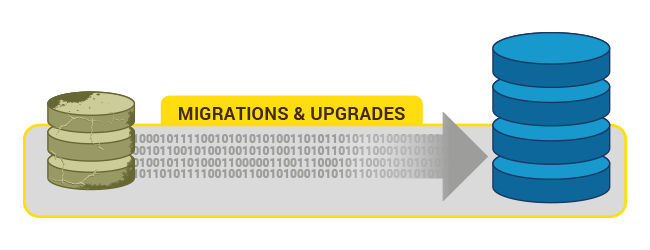
\includegraphics[scale=0.70]{img/pglogical_1.png}\\
\caption{Migrazione e aggiornamenti PostgreSQL \label{figura1} \cite{etichetta3}}
Accumulare le modifiche provenienti da server di database scartati in un data warehouse
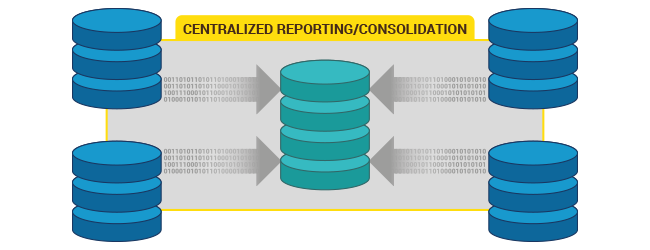
\includegraphics[scale=0.70]{img/pglogical_2.png}\\
\caption{Aggregazione \label{figura2} 
\cite{etichetta4}}
\end{figure}
\begin{figure}[htbp]
\centering
Copiare tutti o una selezione di tabelle di database ad altri nodi di un cluster
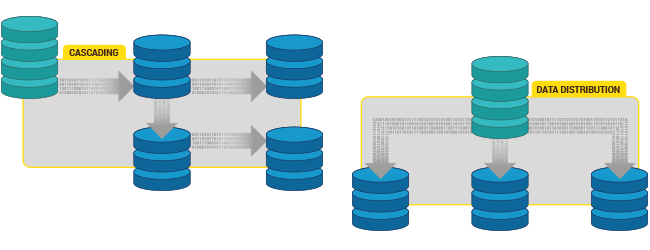
\includegraphics[scale=0.70]{img/pglogical_3.png}\\
\caption{A cascata e distribuzione dati \label{figura3} \cite{etichetta4}}
Le modifiche del database in tempo reale ad altri sistemi
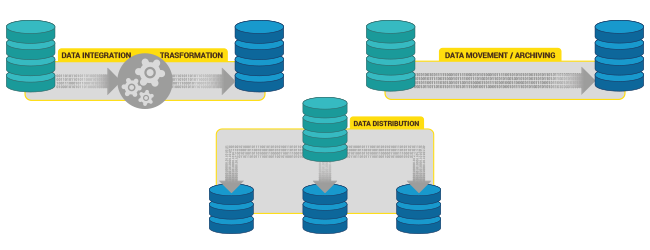
\includegraphics[scale=0.70]{img/pglogical_4.png}\\
\caption{A cascata e distribuzione dati \label{figura4} \cite{etichetta4}}
\end{figure}

\texttt{DA METTERE? DIFFERENZA TRA PG LOGICAL E BDR}
Replica pglogical Bi-Directional Replication (BDR)?
No. pglogical non fornisce funzionalità complete di replica multi-master e un supporto di modifica dello schema coerente, come fa la BDR. Pglogical incorpora le funzionalità di BDR e le lezioni apprese da BDR per produrre una soluzione più semplice e più semplice da utilizzare per la replica unidirezionale, utilizzabile da più persone per una vasta gamma di casi di utilizzo. BDR è stato progettato innanzitutto per il multi-master della rete a n-way, e questo è stato difficile adattarsi bene alla replica mono-master a senso unico.
%\end{document}
